\let\negmedspace\undefined
\let\negthickspace\undefined
\documentclass[journal]{IEEEtran}
\usepackage[a5paper, margin=10mm, onecolumn]{geometry}
%\usepackage{lmodern} % Ensure lmodern is loaded for pdflatex
\usepackage{tfrupee} % Include tfrupee package

\setlength{\headheight}{1cm} % Set the height of the header box
\setlength{\headsep}{0mm}     % Set the distance between the header box and the top of the text

\usepackage{gvv-book}
\usepackage{gvv}
\usepackage{cite}
\usepackage{amsmath,amssymb,amsfonts,amsthm}
\usepackage{algorithmic}
\usepackage{graphicx}
\usepackage{textcomp}
\usepackage{xcolor}
\usepackage{txfonts}
\usepackage{listings}
\usepackage{enumitem}
\usepackage{mathtools}
\usepackage{gensymb}
\usepackage{comment}
\usepackage[breaklinks=true]{hyperref}
\usepackage{tkz-euclide} 
\usepackage{listings}
% \usepackage{gvv}                                        
\def\inputGnumericTable{}                                 
\usepackage[latin1]{inputenc}                                
\usepackage{color}                                            
\usepackage{array}                                            
\usepackage{longtable}                                       
\usepackage{calc}                                             
\usepackage{multirow}                                         
\usepackage{hhline}                                           
\usepackage{ifthen}                                           
\usepackage{lscape}

\begin{document}

\bibliographystyle{IEEEtran}
\vspace{3cm}

\title{2.7.27}
\author{EE25BTECH11015 - Bhoomika V}
% \maketitle
% \newpage
% \bigskip
{\let\newpage\relax\maketitle}

\renewcommand{\thefigure}{\theenumi}
\renewcommand{\thetable}{\theenumi}
\setlength{\intextsep}{10pt} % Space between text and floats


\numberwithin{equation}{enumi}
\numberwithin{figure}{enumi}
\renewcommand{\thetable}{\theenumi}
\parindent 0px 
{Question :-} \\ 
\[
\text{Find the area of the triangle } ABC \text{ whose vertices are }
\vec{A}(2,5),\; \vec{B}(4,7),\; \vec{C}(6,2).
\]

\solution \\
\begin{table}[H]    
  \centering
  \begin{tabular}{|c|c|}
\hline
\textbf{Name} & \textbf{Value} \\ \hline
$\vec{A}$ & $\myvec{2 & 1 \\0 & 3}$ \\ \hline
\end{tabular}

  \caption{Vectors}
  \label{Answers}
\end{table}

\begin{align}
(\vec{A}-\vec{B})
&= \begin{bmatrix} 2 \\ 5 \\ 0 \end{bmatrix}
  - \begin{bmatrix} 4 \\ 7 \\ 0 \end{bmatrix}
= \begin{bmatrix} -2 \\ -2 \\ 0 \end{bmatrix},
\label{eq:AB} \\[6pt]
(\vec{A}-\vec{C})
&= \begin{bmatrix} 2 \\ 5 \\ 0 \end{bmatrix}
  - \begin{bmatrix} 6 \\ 2 \\ 0 \end{bmatrix}
= \begin{bmatrix} -4 \\ 3 \\ 0 \end{bmatrix}.
\label{eq:AC}
\end{align}

Using \eqref{eq:AB} and \eqref{eq:AC}  The magnitude of the cross product is
\begin{align}
\big\lVert (\vec{A}-\vec{B}) \times (\vec{A}-\vec{C}) \big\rVert
&= \sqrt{0^2 + 0^2 + (-14)^2} = 14.
\label{eq:norm}
\end{align}

Therefore the area of triangle \(ABC\) is
\begin{align}
\text{ar}(\triangle ABC)
&= \tfrac{1}{2}\,\big\lVert (\vec{A}-\vec{B}) \times (\vec{A}-\vec{C}) \big\rVert
= \tfrac{1}{2}\times 14 = 7.
\label{eq:area}
\end{align}

     Therefore  \(\displaystyle \text{ar}(\triangle ABC)=7\).
\begin{figure}[H]
\begin{center}
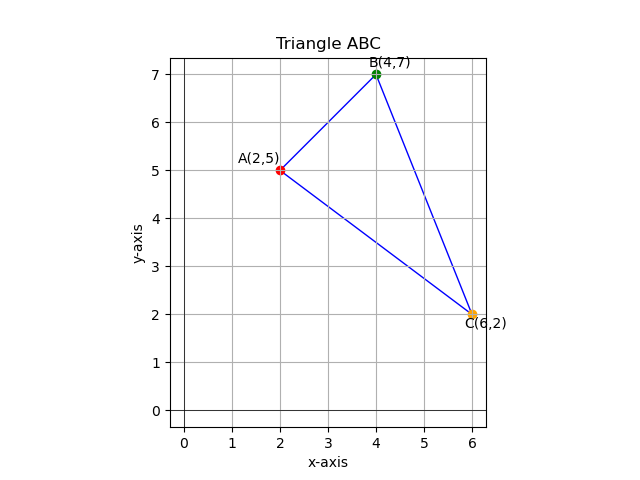
\includegraphics[width=0.6\columnwidth]{Figs/Fig1.png}
\end{center}
\caption{}
\label{fig:Fig.1}
\end{figure}

\end{document}

